\documentclass{article}
\usepackage{amsmath,amssymb}
\usepackage{geometry}
\usepackage{pgfplots}
\pgfplotsset{compat=1.16}
\title{PHYSICS 531 Honor Project}
\author{Yufei Shen}
\date{Aug 18, 2025}
\begin{document}
    \maketitle
    \section{Problem 1: Bulk Dirac Equation in 2 and 3 Spatial Dimensions}

    To determine the energy eigenvalues of the Hamiltonians specified in Problem 1, we transition from a position-space representation to a momentum-space representation using the Fourier transform. The wavefunction $\Psi(\mathbf{r})$ is expressed as a superposition of plane waves:
    \begin{equation}
        \Psi(\mathbf{r}) = \int \frac{d^D p}{(2\pi)^D}\, e^{i\mathbf{p}\cdot \mathbf{r}}\, \tilde{\Psi}(\mathbf{p}),
    \end{equation}
    where $D$ is the spatial dimension (2 or 3), $\mathbf{p}$ is the momentum vector, and $\tilde{\Psi}(\mathbf{p})$ is the momentum-space wavefunction. In this basis, the momentum operator $\hat{\mathbf{p}} = -i\nabla$ (we set $\hbar=1$ in this section) acting on $\Psi(\mathbf{r})$ becomes multiplication by the vector $\mathbf{p}$ for $\tilde{\Psi}(\mathbf{p})$.

    The eigenvalue equation for the Hamiltonian $\hat{H}$ in position space, $\hat{H}\Psi(\mathbf{r}) = E\Psi(\mathbf{r})$, transforms into an algebraic eigenvalue problem in momentum space:
    \begin{equation}
        H(\mathbf{p})\tilde{\Psi}(\mathbf{p}) = E(\mathbf{p})\tilde{\Psi}(\mathbf{p}).
    \end{equation}
    Here, $H(\mathbf{p})$ is the Hamiltonian matrix expressed in terms of momentum components $\mathbf{p}$, and $E(\mathbf{p})$ are the corresponding energy eigenvalues. These eigenvalues are found by diagonalizing the matrix $H(\mathbf{p})$.

    Both Hamiltonians of Problem 1 have the form
    \begin{equation}
        H(\mathbf{p}) = v \sum_{a} d_a(\mathbf{p})\, \Gamma_a, \qquad \mathbf{d} = (p_1,\dots,p_D, m),
    \end{equation}
    where in 2D $(\Gamma_1,\Gamma_2,\Gamma_3) = (\sigma_x,\sigma_y,\sigma_z)$ and in 3D $(\Gamma_1,\dots,\Gamma_4) = (\beta_x,\beta_y,\beta_z,\alpha)$. In both cases the matrices mutually anticommute and square to the identity, $\{\Gamma_a,\Gamma_b\} = 2\delta_{ab}\mathbb{I}$. Squaring $H$, all cross terms cancel:
    \begin{equation}
        H(\mathbf{p})^2 = v^2 \sum_{a,b} d_a d_b\, \tfrac{1}{2}\{\Gamma_a,\Gamma_b\} = v^2\left(|\mathbf{p}|^2 + m^2\right)\mathbb{I}.
    \end{equation}
    Hence every eigenvalue obeys $E^2 = v^2(|\mathbf{p}|^2+m^2)$, and since $\mathrm{Tr}\,H = 0$ both signs occur equally often:
    \begin{equation} \label{eq:general_eigenvalue}
        E_{\pm}(\mathbf{p}) = \pm v h, \qquad h \equiv \sqrt{|\mathbf{p}|^2 + m^2}.
    \end{equation}
    The $\pm$ signs distinguish between particle and anti-particle solutions (or upper and lower energy bands). The eigenstates do not depend on $v$; below we set $v=1$ where convenient.

    \paragraph{2D Case:}
    With $\mathbf{p} = (p_x, p_y)$,
    \begin{equation}
        H(\mathbf{p}) = \begin{pmatrix} m & p_x - i p_y \\ p_x + i p_y & -m \end{pmatrix}, \qquad E_\pm = \pm\sqrt{p_x^2 + p_y^2 + m^2}.
    \end{equation}
    From the second row, $(p_x+ip_y)a - m b = E b$, the normalized eigenstates are
    \begin{equation} \label{eq:2D_states}
        \psi_{E_+} (\mathbf{p}) = \frac{1}{\sqrt{2h(h + m)}}
        \begin{pmatrix}
            h + m \\
            p_x + i p_y
        \end{pmatrix}, \qquad
        \psi_{E_-} (\mathbf{p}) = \frac{1}{\sqrt{2h(h - m)}}
        \begin{pmatrix}
            m - h \\
            p_x + i p_y
        \end{pmatrix},
    \end{equation}
    where the normalization follows from $(h \pm m)^2 + p_x^2 + p_y^2 = 2h(h\pm m)$. Each band is non-degenerate.

    \paragraph{3D Case:}
    Four mutually anticommuting matrices require dimension 4. A convenient choice is
    \begin{equation}
        \beta_i = \tau_x \otimes \sigma_i, \qquad \alpha = \tau_z \otimes \mathbb{I},
    \end{equation}
    where $\tau_i$ are Pauli matrices in an additional ``orbital'' space. Indeed $\{\beta_i,\beta_j\} = \mathbb{I}\otimes\{\sigma_i,\sigma_j\} = 2\delta_{ij}$, $\{\beta_i,\alpha\} = \{\tau_x,\tau_z\}\otimes\sigma_i = 0$ and $\alpha^2 = \mathbb{I}$. (Any other choice is unitarily equivalent, so the spectrum does not depend on it.) Then
    \begin{equation}
        H(\mathbf{p}) = \begin{pmatrix} m\,\mathbb{I} & \boldsymbol{\sigma}\cdot\mathbf{p} \\ \boldsymbol{\sigma}\cdot\mathbf{p} & -m\,\mathbb{I} \end{pmatrix}, \qquad E_\pm = \pm\sqrt{p_x^2 + p_y^2 + p_z^2 + m^2}.
    \end{equation}
    Using $(\boldsymbol{\sigma}\cdot\mathbf{p})^2 = |\mathbf{p}|^2$, one checks directly that
    \begin{equation}
        \psi_{E_+,s} = \frac{1}{\sqrt{2h(h+m)}}\begin{pmatrix} (h+m)\,\chi_s \\ (\boldsymbol{\sigma}\cdot\mathbf{p})\,\chi_s \end{pmatrix}, \qquad
        \psi_{E_-,s} = \frac{1}{\sqrt{2h(h+m)}}\begin{pmatrix} -(\boldsymbol{\sigma}\cdot\mathbf{p})\,\chi_s \\ (h+m)\,\chi_s \end{pmatrix},
    \end{equation}
    with $\chi_\uparrow = (1,0)^T$, $\chi_\downarrow = (0,1)^T$. Each energy level is therefore doubly degenerate.

    \subsection{Eigenstates, Berry Connection, and Curvature for the 2D Hamiltonian}
    We now return to the 2D Hamiltonian, $H = \mathbf{h}(\mathbf{p}) \cdot \vec{\sigma}$ with $\mathbf{h}(\mathbf{p}) = (p_x, p_y, m)$ and $h = |\mathbf{h}|$. Writing $p_x + i p_y = p\, e^{i\phi}$, the eigenstates of Eq.~\eqref{eq:2D_states} read
    \begin{equation}
        \psi_{E_+} = \frac{1}{\sqrt{2h(h + m)}}\begin{pmatrix} h + m \\ p\, e^{i\phi} \end{pmatrix}, \qquad
        \psi_{E_-} = \frac{1}{\sqrt{2h(h - m)}}\begin{pmatrix} m - h \\ p\, e^{i\phi} \end{pmatrix}.
    \end{equation}
    (In this gauge $\psi_{E_+}$ is singular at $p=0$ when $m<0$, and $\psi_{E_-}$ when $m>0$, because the phase $e^{i\phi}$ is undefined there. This is a gauge artifact: multiplying by $e^{-i\phi}$ moves the singularity to $p\to\infty$. The gauge-invariant Berry curvature below is smooth everywhere.)

    Since the normalization and the first component are real, only the phase $e^{i\phi}$ contributes to the Berry connection $\mathcal{A}_i = i \langle \psi | \partial_{p_i} \psi \rangle$:
    \begin{equation}
        \boldsymbol{\mathcal{A}}^{\pm} = -|\psi_{E_\pm,2}|^2\, \nabla_{\mathbf{p}}\phi
        = -\frac{h \mp m}{2h}\,\nabla_{\mathbf{p}}\phi, \qquad \nabla_{\mathbf{p}}\phi = \frac{(-p_y,\, p_x)}{p^2},
    \end{equation}
    where we used $p^2 = (h-m)(h+m)$. For the upper band this gives
    \begin{equation}
        \mathcal{A}^+_x(\mathbf{p}) = \frac{p_y}{2h(h+m)}, \quad
        \mathcal{A}^+_y(\mathbf{p}) = \frac{-p_x}{2h(h+m)}.
    \end{equation}
    The Berry curvature $\Omega = \epsilon_{ij}\partial_{p_i}\mathcal{A}_j$ is
    \begin{equation}
        \Omega(\mathbf{p}) = \frac{\partial \mathcal{A}_y}{\partial p_x} - \frac{\partial \mathcal{A}_x}{\partial p_y}.
    \end{equation}
    For a connection of the form $\boldsymbol{\mathcal{A}} = a(p)\nabla\phi$ this reduces to $\Omega = \frac{1}{p}\frac{da}{dp}$. With $a_\pm = -\frac{1}{2} \pm \frac{m}{2h}$ and $dh/dp = p/h$:
    \begin{equation}
        \Omega_{\pm}(\mathbf{p}) = \mp\frac{m}{2h^3} = \mp\frac{m}{2(p_x^2 + p_y^2 + m^2)^{3/2}}.
    \end{equation}
    As required for a two-band model, $\Omega_+ + \Omega_- = 0$.

    We now calculate the requested integral. Converting to polar coordinates ($d^2p = p \,dp \,d\phi$):
    \begin{align}
        \int \frac{d^2p}{(2\pi)^2}\, \Omega_\pm(\mathbf{p}) &= \mp\frac{1}{(2\pi)^2}\int_0^{2\pi} d\phi \int_0^{\infty} p \,dp \, \frac{m}{2(p^2 + m^2)^{3/2}}
        = \mp\frac{m}{4\pi} \int_0^{\infty} \frac{p}{(p^2 + m^2)^{3/2}} \,dp.
    \end{align}
    To evaluate the integral, let $u = p^2 + m^2$, so $du = 2p \,dp$. When $p=0$, $u=m^2$. When $p\to\infty$, $u\to\infty$.
    \begin{align}
        \int_0^{\infty} \frac{p}{(p^2 + m^2)^{3/2}} \,dp &= \frac{1}{2} \int_{m^2}^{\infty} u^{-3/2} \,du
        = \frac{1}{2} \left[ -2u^{-1/2} \right]_{m^2}^{\infty} = \frac{1}{|m|}.
    \end{align}
    Therefore
    \begin{equation}
        \int \frac{d^2p}{(2\pi)^2}\, \Omega_\pm(\mathbf{p}) = \mp\frac{\mathrm{sign}(m)}{4\pi}.
    \end{equation}
    The Chern number of band $n$ is $C_n = \frac{1}{2\pi}\int d^2p\, \Omega_n$, i.e.\ $2\pi$ times the integral above:
    \begin{equation}
        C_\pm = \mp\frac{1}{2}\mathrm{sign}(m).
    \end{equation}
    The physically relevant band is the filled lower band (Fermi level in the gap), with $C_- = +\frac{1}{2}\mathrm{sign}(m)$. The measure $d^2p/(2\pi)^2$ appears naturally in the Hall conductance (TKNN/Kubo formula):
    \begin{equation}
        \sigma_{xy} = \frac{e^2}{\hbar}\int \frac{d^2p}{(2\pi)^2}\, \Omega_-(\mathbf{p}) = \frac{e^2}{h}\, C_- = \mathrm{sign}(m)\,\frac{e^2}{2h}.
    \end{equation}
    If $m=0$, the result is ill-defined as the gap closes.

    \paragraph{Why a half-integer?} A Chern number of a band over a closed Brillouin zone must be an integer. In the continuum model, however, the unit vector $\hat{\mathbf{h}}(\mathbf{p})$ only covers one hemisphere of the sphere as $\mathbf{p}$ ranges over $\mathbb{R}^2$ (it points to a pole at $p=0$ and to the equator as $p\to\infty$), and $|C|$ equals the covered solid angle divided by $4\pi$. A lattice regularization fixes the behaviour at large $p$, e.g.\ $m \to m - Bp^2$, which gives $C_- = \frac{1}{2}[\mathrm{sign}(m) + \mathrm{sign}(B)] \in \{0, \pm 1\}$. The regularization-independent statement is the \emph{change} $|C_-(m>0) - C_-(m<0)| = 1$ when the mass changes sign. This is exactly what guarantees the single edge mode of Problem 2.

    \section{Problem 2: Edge States of 2D Dirac Hamiltonian}
	We consider the 2D Dirac Hamiltonian of Eq.~(1) with a mass term $m(y)$ that varies along the $y$-direction, creating an interface. Such a system can host chiral edge states, as described by Jackiw and Rebbi~\cite{JR} and found in topological insulators (Hasan and Kane review~\cite{HK}, Eq.~6).
	
	The reference solution (Eq.~6 in Hasan and Kane) is of the form:
	\begin{equation} \label{eq:kane_hazan_6_main}
		\psi_{q_x}(x,y) = \mathcal{N} e^{i q_x x} \exp\left(-\int_0^y \frac{m(y')}{\hbar v_F} dy'\right) \begin{pmatrix} 1 \\ 1 \end{pmatrix},
	\end{equation}
	with a linear energy dispersion relation:
	\begin{equation} \label{eq:edge_dispersion_main}
		E(q_x) = \hbar v_F q_x.
	\end{equation}
	Here, $q_x$ is the wavevector along the edge (x-direction), $v_F$ is the Fermi velocity, and $\mathcal{N}$ is a normalization constant. In the review, $m(y)$ changes sign across $y=0$ ($m(y) < 0$ for $y<0$ and $m(y) > 0$ for $y>0$).
	
	\subsection{Derivation of the Edge State}
	We use Eq.~(1) with $m \to m(y)$ (absorbing $v_F$ into $m(y)$, so that $m(y)$ has units of energy as in the review):
	\begin{equation}
		H = v_F (\hat{p}_x \sigma_x + \hat{p}_y \sigma_y) + m(y) \sigma_z,
	\end{equation}
	where $\hat{p}_x = -i\hbar\partial_x$, $\hat{p}_y = -i\hbar\partial_y$, and $\sigma_i$ are the standard Pauli matrices.
	We look for a solution of the form $\psi(x,y) = e^{i q_x x} \Phi(y)$. Substituting $\hat{p}_x \to \hbar q_x$:
	\begin{equation}
		H \psi = \left[ v_F (\hbar q_x \sigma_x + (-i\hbar\partial_y) \sigma_y) + m(y) \sigma_z \right] e^{i q_x x} \Phi(y) = E e^{i q_x x} \Phi(y).
	\end{equation}
	We propose an ansatz for the spinor part $\Phi(y) = \phi(y) \chi$, where $\chi = \begin{pmatrix} 1 \\ 1 \end{pmatrix}$. This spinor is an eigenstate of $\sigma_x$ with eigenvalue $+1$: $\sigma_x \chi = \chi$.
	The eigenvalue equation becomes:
	\begin{equation}
		\left[ v_F \hbar q_x \sigma_x - i \hbar v_F \sigma_y \partial_y + m(y) \sigma_z \right] \phi(y) \chi = E \phi(y) \chi.
	\end{equation}
	We are looking for states with the dispersion $E = \hbar v_F q_x$. Substituting this and using $\sigma_x \chi = \chi$, the $q_x$ terms cancel and we obtain
	\begin{equation}
		\left( -i \hbar v_F \sigma_y \partial_y + m(y) \sigma_z \right) \phi(y) \chi = 0.
	\end{equation}
	Expanding $\partial_y (\phi(y)\chi) = (\partial_y \phi) \chi$ (since $\chi$ is $y$-independent):
	\begin{equation}
		-i \hbar v_F (\partial_y \phi) \sigma_y \chi + m(y) \phi \sigma_z \chi = 0.
	\end{equation}
	We calculate the action of Pauli matrices on $\chi = \begin{pmatrix} 1 \\ 1 \end{pmatrix}$:
	\begin{align*}
		\sigma_y \chi &= \begin{pmatrix} 0 & -i \\ i & 0 \end{pmatrix} \begin{pmatrix} 1 \\ 1 \end{pmatrix} = \begin{pmatrix} -i \\ i \end{pmatrix} = i \begin{pmatrix} -1 \\ 1 \end{pmatrix}, \\
		\sigma_z \chi &= \begin{pmatrix} 1 & 0 \\ 0 & -1 \end{pmatrix} \begin{pmatrix} 1 \\ 1 \end{pmatrix} = \begin{pmatrix} 1 \\ -1 \end{pmatrix}.
	\end{align*}
	Substituting these into the equation:
	\begin{equation}
		-i \hbar v_F (\partial_y \phi) \left(i \begin{pmatrix} -1 \\ 1 \end{pmatrix}\right) + m(y) \phi \begin{pmatrix} 1 \\ -1 \end{pmatrix} = 0.
	\end{equation}
	This can be rewritten as:
	\begin{equation}
		\left( -\hbar v_F (\partial_y \phi) + m(y) \phi \right) \begin{pmatrix} 1 \\ -1 \end{pmatrix} = 0.
	\end{equation}
	For a non-trivial solution, we require the scalar part to be zero:
	\begin{equation}
		\frac{d\phi}{dy} = +\frac{m(y)}{\hbar v_F} \phi(y),
	\end{equation}
	with solution
	\begin{equation} \label{eq:our_edge_state}
		\phi(y) = \mathcal{N} \exp\left(+\int_0^y \frac{m(y')}{\hbar v_F} dy'\right).
	\end{equation}

	\paragraph{Comparison with Eq.~(6) of the review.} With the sign convention of Eq.~(1), our result differs from Eq.~(6) by $m(y) \to -m(y)$: the state $\propto (1,1)^T$ with $E = +\hbar v_F q_x$ is bound to a wall with $m>0$ for $y<0$ and $m<0$ for $y>0$. Repeating the same steps with $\chi = (1,-1)^T$ ($\sigma_x\chi = -\chi$) gives $\phi \propto \exp(-\int_0^y m/\hbar v_F)$ with $E = -\hbar v_F q_x$. So the wall of the review ($m>0$ for $y>0$) binds a mode of the \emph{opposite} chirality in our convention. Equation~(6) is reproduced literally if the $\sigma_y$ term enters with the opposite sign, $v_F(\hat p_x\sigma_x - \hat p_y\sigma_y)$. The physics is identical: one chiral mode bound where the mass changes sign, with direction set by the sign of the mass jump.

	\paragraph{Normalization and Localization:}
	For the state to be a localized edge state, $\phi(y)$ must decay as $y \to \pm\infty$. For Eq.~\eqref{eq:our_edge_state} this requires $\int_0^y m(y')dy' \to -\infty$ for $y\to+\infty$ and $\to +\infty$ for $y \to -\infty$.
	Consider a mass domain wall $m(y) = -m_0 \,\mathrm{sgn}(y)$ with $m_0 > 0$.
	Then $\int_0^y \frac{m(y')}{\hbar v_F} dy' = -\frac{m_0}{\hbar v_F} |y|$, and
	\begin{equation}
		\psi_{q_x}(x,y) = \sqrt{\frac{m_0}{2\hbar v_F}}\; e^{i q_x x} \exp\left(-\frac{m_0|y|}{\hbar v_F}\right)\begin{pmatrix} 1 \\ 1 \end{pmatrix},
	\end{equation}
	normalized per unit length along $x$. This state is localized at $y=0$ within the length $\hbar v_F/m_0$.

	\paragraph{Bulk-boundary correspondence:} Far from the wall the system is a gapped bulk with $C_- = +\frac{1}{2}$ on one side and $C_- = -\frac{1}{2}$ on the other (Problem 1). The jump $|\Delta C| = 1$ equals the number of chiral modes found at the interface.

	\subsection{Dispersion Plot for Bulk and Edge States}
	The following plot illustrates the bulk energy bands for a 2D Dirac material and the linearly dispersing chiral edge state that appears at an interface where the mass term $m$ changes sign, as in Fig.~2(b) of Ref.~\cite{HK}. We set $\hbar=1$, $v_F=1$, and a representative mass $m_0=0.5$ for the bulk gap. For a given $q_x$, bulk states exist at $E = \pm\sqrt{q_x^2 + p_y^2 + m_0^2}$ for every $p_y$; the band edges ($p_y=0$) are shown in blue and the continuum ($p_y\neq0$) in gray. The edge state dispersion is $E=q_x$, which connects the lower and upper bulk bands across the gap.

	\begin{figure}[h]
		\centering
		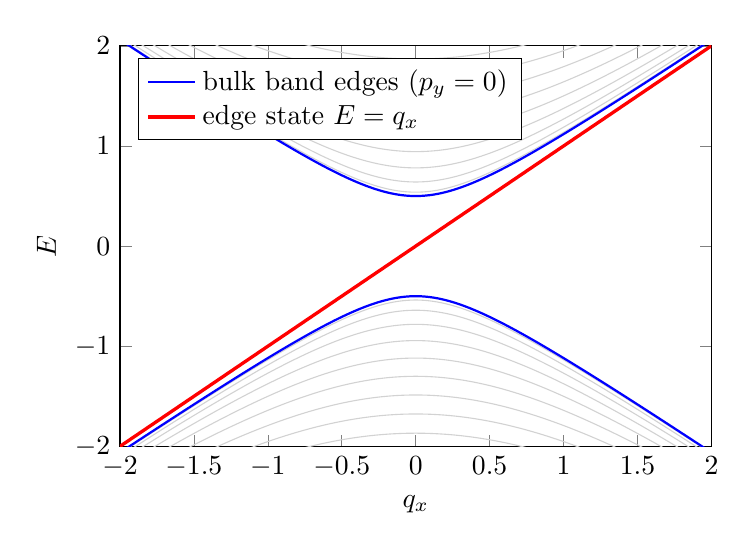
\begin{tikzpicture}
			\begin{axis}[
				width=0.75\textwidth, height=0.55\textwidth,
				xlabel={$q_x$}, ylabel={$E$},
				xmin=-2, xmax=2, ymin=-2, ymax=2,
				domain=-2:2, samples=150,
				legend pos=north west, legend cell align=left]
				\pgfplotsinvokeforeach{1,...,10}{
					\addplot[gray!35, forget plot] {sqrt(x^2 + (#1*0.2)^2 + 0.25)};
					\addplot[gray!35, forget plot] {-sqrt(x^2 + (#1*0.2)^2 + 0.25)};
				}
				\addplot[blue, thick] {sqrt(x^2 + 0.25)};
				\addlegendentry{bulk band edges ($p_y=0$)}
				\addplot[blue, thick, forget plot] {-sqrt(x^2 + 0.25)};
				\addplot[red, very thick] {x};
				\addlegendentry{edge state $E = q_x$}
			\end{axis}
		\end{tikzpicture}
		\caption{Bulk bands (blue and gray) of the 2D Dirac Hamiltonian with $m_0 = 0.5$ and the chiral edge state (red) bound to the mass domain wall.}
	\end{figure}

    \section{Problem 3: 1D Dirac Equation and Fermion Number Fractionalization}
    Setting $p_x = 0$ in Eq.~(1) with $m \to m(y)$ (and $\hbar = v = 1$) gives the 1D Dirac Hamiltonian
    \begin{equation}
        H_{1D} = -i\sigma_y\partial_y + m(y)\sigma_z.
    \end{equation}

    \paragraph{Uniform mass.} For constant $m$, plane waves $e^{iky}$ give $H(k) = k\sigma_y + m\sigma_z$, i.e.\ the 2D result with $(p_x, p_y) \to (0,k)$:
    \begin{equation}
        E_\pm(k) = \pm\sqrt{k^2+m^2}, \qquad \psi_{E_+} = \frac{1}{\sqrt{2h(h + m)}}\begin{pmatrix} h + m \\ ik \end{pmatrix}, \qquad
        \psi_{E_-} = \frac{1}{\sqrt{2h(h - m)}}\begin{pmatrix} m - h \\ ik \end{pmatrix}.
    \end{equation}

    \paragraph{Domain wall.} For $m(y) = -m_0\,\mathrm{sgn}(y)$, there are continuum (scattering) states with $E = \pm\sqrt{k^2 + m_0^2}$ and, in addition, exactly one bound state at $E=0$. This is the $q_x=0$ member of the edge state of Problem 2:
    \begin{equation}
        \psi_0(y) = \sqrt{\frac{m_0}{2}}\, e^{-m_0|y|}\begin{pmatrix} 1 \\ 1 \end{pmatrix}, \qquad H_{1D}\psi_0 = 0.
    \end{equation}
    The spectrum is symmetric: since $\sigma_x\sigma_y\sigma_x = -\sigma_y$ and $\sigma_x\sigma_z\sigma_x = -\sigma_z$, we have $\sigma_x H_{1D} \sigma_x = -H_{1D}$. Thus every state $\psi_E$ has a partner $\sigma_x\psi_E$ at energy $-E$, while the zero mode is its own partner, $\sigma_x\psi_0 = \psi_0$.

    \paragraph{Counting the fermion number.} Following Jackiw and Rebbi~\cite{JR}, we use the charge-conjugation-symmetric fermion number operator $N = \frac{1}{2}\int dy\, [\psi^\dagger, \psi]$. Expanding the field in the eigenmodes of $H_{1D}$ gives, for a many-body state with occupation numbers $n_E \in \{0,1\}$,
    \begin{equation}
        N = \sum_E \left(n_E - \tfrac{1}{2}\right) = \frac{1}{2}\Big(\sum_{\text{filled}} 1 - \sum_{\text{empty}} 1\Big).
    \end{equation}
    For a uniform system with the Dirac sea filled, the symmetric spectrum gives $N=0$, so $N$ measures the fermion number relative to the vacuum. In the presence of the wall we fill all $E<0$ states. The continuum then contributes $\frac{1}{2}\left(\#\{E<0\} - \#\{E>0\}\right) = 0$ by the $E \leftrightarrow -E$ symmetry, and the zero mode contributes $n_0 - \frac{1}{2}$:
    \begin{equation}
        N = n_0 - \tfrac{1}{2} = \pm\tfrac{1}{2}.
    \end{equation}
    The same result follows by summing over the filled states directly. Let $\Delta\rho(E) = \rho_{\text{wall}}(E) - \rho_{\text{uniform}}(E) = \delta(E) + \Delta\rho_c(E)$. The wall does not change the total number of states, so $\int dE\, \Delta\rho(E) = 0$. Spectral symmetry gives $\Delta\rho_c(E) = \Delta\rho_c(-E)$, hence
    \begin{equation}
        \int_{-\infty}^{0^-} dE\, \Delta\rho_c(E) = -\tfrac{1}{2}.
    \end{equation}
    The zero mode is built half from negative-energy and half from positive-energy continuum states. The filled Dirac sea therefore contains half a state less than without the wall, and the total fermion number is $N = -\frac{1}{2} + n_0 = \pm\frac{1}{2}$. Since the system looks uniform far from the wall, this charge is localized within $\sim 1/m_0$ of $y=0$.

    \paragraph{Fractionalization of fermion:}
    Fermion number fractionalization occurs when a topological defect, such as a mass domain wall in a Dirac system, hosts a localized zero-energy electronic state. This special state, positioned exactly between occupied negative-energy states (like the Dirac sea) and empty positive-energy states, results in the defect effectively binding a non-integer fermion number, $\pm 1/2$, compared to a system without such a defect. Consequently, the defect itself appears to carry a fractional charge or fermion number within the material's collective electronic ground state, even though fundamental fermions remain indivisible. The value is pinned exactly to $\pm1/2$ by the $E\leftrightarrow -E$ symmetry. For electrons with spin (e.g.\ solitons in polyacetylene, the Su--Schrieffer--Heeger model~\cite{SSH}) the factor of 2 makes the charge an integer, but leads to unusual spin--charge relations: charged solitons without spin and neutral solitons with spin $1/2$.

    \section{Problem 4: Topological Insulators and Summary}
    \paragraph{Literature: Chern insulators and the quantum anomalous Hall effect.}
    Thouless, Kohmoto, Nightingale and den Nijs (TKNN)~\cite{TKNN} showed that the Hall conductance of a filled band in a 2D crystal is $e^2/h$ times an integer, the Chern number of that band. Haldane~\cite{Haldane} constructed a honeycomb-lattice model with zero net magnetic flux but broken time-reversal symmetry that has a quantized Hall conductance without Landau levels: a Chern insulator, whose Hall response is called the quantum anomalous Hall (QAH) effect. Near the two Dirac points $K$, $K'$ the low-energy Hamiltonian is Eq.~(1) with masses $m_K$, $m_{K'}$. Because the two valleys have opposite chirality, each contributes $\pm\frac{1}{2}\mathrm{sign}(m)$ with opposite signs, so $C = \frac{1}{2}[\mathrm{sign}(m_K) - \mathrm{sign}(m_{K'})]$ (up to an overall sign convention). Equal masses (inversion breaking) give a trivial insulator, while opposite masses (Haldane's time-reversal breaking term) give $|C| = 1$. This is the lattice resolution of the half-integer found in Problem 1. A simpler square-lattice two-band model was introduced by Qi, Wu and Zhang~\cite{QWZ}, $\mathbf{h}(\mathbf{k}) = (\sin k_x, \sin k_y, m - \cos k_x - \cos k_y)$, which has $|C|=1$ for $0<|m|<2$ and $C=0$ for $|m|>2$; near $\mathbf{k}=0$ it reduces to Eq.~(1) with the regularized mass $m - 2 + k^2/2$. Yu \emph{et al.}~\cite{Yu} predicted the QAH effect in magnetically doped thin films of the Bi$_2$Se$_3$ family, and Chang \emph{et al.}~\cite{Chang} observed it in Cr-doped (Bi,Sb)$_2$Te$_3$ films: a Hall resistance quantized at $h/e^2$ in zero magnetic field with nearly vanishing longitudinal resistance, at temperatures of tens of millikelvin.

    \paragraph{Berry curvature, Berry connection, Chern number:} The Berry connection describes the geometric phase acquired by a quantum state as parameters are varied adiabatically; its curl is the Berry curvature, and the integral of this curvature over the Brillouin zone gives the Chern number, a topological invariant characterizing electronic bands. The Chern number of the filled bands determines the quantized Hall conductance $\sigma_{xy} = C e^2/h$~\cite{TKNN, XCN}.

    \paragraph{Bulk-Boundary correspondence:} This principle states that the non-trivial topological properties of a material's bulk (e.g., a non-zero Chern number) necessitate the existence of protected, gapless states at its boundaries or edges. Quantitatively, the net number of chiral edge modes at an interface equals the difference of the bulk Chern numbers on the two sides, $|\Delta C|$; for the domain wall of Problem 2, $|\Delta C| = 1$ and we found exactly one chiral mode.

    \paragraph{Edge states and why they are robust:} Edge states are electronic states localized at the boundary of a material, often with unique transport properties; they are robust because their existence is guaranteed by the bulk topology, making them insensitive to local perturbations that do not close the bulk gap or break fundamental symmetries. In a Chern insulator the edge modes are chiral: on a given edge all of them move in the same direction, so there is no state to backscatter into, and disorder cannot localize them.

    \paragraph{Dirac equation in solid-state systems and the sign of the mass:} In some solid-state systems (like graphene or topological insulators), the electron energy-momentum relationship near certain points (Dirac points) becomes linear, mimicking the massless Dirac equation; a gap can be opened, leading to an effective mass term which can be positive or negative depending on the band structure details (e.g., band inversion), distinguishing trivial from topological phases. The mass is the energy difference between two bands (e.g.\ $s$- and $p$-like orbitals) at the gap minimum, so it changes sign when the band ordering is inverted, for instance by spin--orbit coupling or film thickness. Only the sign of the mass \emph{relative} to the band curvature at large momentum ($B$ in $m - Bk^2$) is meaningful, and it decides whether $C=0$ or $|C|=1$.

    \begin{thebibliography}{99}
        \bibitem{HK} M. Z. Hasan and C. L. Kane, ``Colloquium: Topological insulators,'' Rev.\ Mod.\ Phys.\ \textbf{82}, 3045 (2010).
        \bibitem{BH} B. A. Bernevig and T. L. Hughes, \emph{Topological Insulators and Topological Superconductors} (Princeton University Press, 2013).
        \bibitem{JR} R. Jackiw and C. Rebbi, ``Solitons with fermion number 1/2,'' Phys.\ Rev.\ D \textbf{13}, 3398 (1976).
        \bibitem{XCN} D. Xiao, M.-C. Chang, and Q. Niu, ``Berry phase effects on electronic properties,'' Rev.\ Mod.\ Phys.\ \textbf{82}, 1959 (2010).
        \bibitem{TKNN} D. J. Thouless, M. Kohmoto, M. P. Nightingale, and M. den Nijs, Phys.\ Rev.\ Lett.\ \textbf{49}, 405 (1982).
        \bibitem{Haldane} F. D. M. Haldane, Phys.\ Rev.\ Lett.\ \textbf{61}, 2015 (1988).
        \bibitem{QWZ} X.-L. Qi, Y.-S. Wu, and S.-C. Zhang, Phys.\ Rev.\ B \textbf{74}, 085308 (2006).
        \bibitem{Yu} R. Yu, W. Zhang, H.-J. Zhang, S.-C. Zhang, X. Dai, and Z. Fang, Science \textbf{329}, 61 (2010).
        \bibitem{Chang} C.-Z. Chang \emph{et al.}, Science \textbf{340}, 167 (2013).
        \bibitem{SSH} W. P. Su, J. R. Schrieffer, and A. J. Heeger, Phys.\ Rev.\ Lett.\ \textbf{42}, 1698 (1979).
    \end{thebibliography}

\end{document}
